\documentclass[12pt]{report} %[span_3](start_span)[span_3](end_span)

\usepackage{suproposal} %[span_4](start_span)[span_4](end_span)
\usepackage{enumitem} %[span_5](start_span)[span_5](end_span)
\setlist[itemize]{itemsep=0.5pt, topsep=1pt} %[span_6](start_span)[span_6](end_span)

\usepackage{tikz} %[span_7](start_span)[span_7](end_span)
\usetikzlibrary{positioning,arrows.meta} %[span_8](start_span)[span_8](end_span)

\hypersetup{ %[span_9](start_span)[span_9](end_span)
	pdfencoding=auto,
	pdfauthor={Dương Đình Phương Dao},
	pdfsubject={Khoa học máy tính},
	pdftitle={Phát hiện, lý giải và can thiệp bất thường trong hình ảnh AI tạo sinh}
}

\begin{document}

\firstbeforepreface %[span_10](start_span)[span_10](end_span)
\setcounter{page}{1} %[span_11](start_span)[span_11](end_span)
\newpage %[span_12](start_span)[span_12](end_span)
\afterpreface %[span_13](start_span)[span_13](end_span)

\section{Giới thiệu bài toán}
\label{sec:intro} %[span_14](start_span)[span_14](end_span)

\subsection{Bối cảnh thực tiễn}
Sự phát triển của các mô hình học máy tạo sinh (AI-Generated Content - AIGC), nổi bật là Mạng đối kháng tạo sinh (GAN) và mô hình Khuếch tán (Diffusion Models), đã tạo ra bước ngoặt trong việc tổng hợp nội dung thị giác~\cite{yin2023generative}. %[span_15](start_span)[span_15](end_span)[span_16](start_span)[span_16](end_span) Tuy nhiên, một rào cản kỹ thuật cốt lõi làm suy giảm tính chân thực và cản trở triển khai trong các ứng dụng thương mại chính là sự xuất hiện của các "bất thường thị giác" (visual anomalies hay generative artifacts)~\cite{cao2024synartifact}. %[span_17](start_span)[span_17](end_span)[span_18](start_span)[span_18](end_span) Việc giải quyết hiện tượng này đóng vai trò quyết định trong việc vượt qua "thung lũng kỳ lạ" (uncanny valley) của hình ảnh AI. %[span_19](start_span)[span_19](end_span)

\subsection{Định nghĩa bài toán}
Trong xử lý ảnh truyền thống, sự suy giảm chất lượng ảnh thường được mô hình hóa dưới dạng nhiễu cộng tuyến tính. Ngược lại, bất thường tạo sinh (AIGC Anomalies) có bản chất toán học phức tạp hơn: chúng là sự lệch lạc trong quá trình dựng đa tạp nội suy~\cite{yin2023generative}. %[span_20](start_span)[span_20](end_span)[span_21](start_span)[span_21](end_span) Bài toán mà đề tài tập trung giải quyết là \textbf{Intent-aware In-Situ Anomaly Correction (Can thiệp bất thường tại chỗ nhận biết ý định)}. %[span_22](start_span)[span_22](end_span) 
\begin{itemize}
    \item \textbf{Đầu vào:} Quá trình tạo sinh đang diễn ra với câu lệnh văn bản gốc ($P$) và quỹ đạo tiềm ẩn (latent trajectory) tại bước thời gian $t$. %[span_23](start_span)[span_23](end_span)
    \item \textbf{Đầu ra:} Hình ảnh cuối cùng ($I_{corr}$) đã được ngăn chặn các artifact từ giai đoạn lấy mẫu, phục hồi tính logic vật lý nhưng bảo toàn tuyệt đối ý định sáng tạo ban đầu của người dùng (bao gồm cả các ý định siêu thực). %[span_24](start_span)[span_24](end_span)
\end{itemize}

\subsection{Các thách thức chính}
Việc phát hiện và chỉnh sửa bất thường đối mặt với ba thách thức khoa học cốt lõi: %[span_25](start_span)[span_25](end_span)
\begin{itemize}
    \item \textbf{Bản chất phi tuyến tính của lỗi:} Các lỗi trải dài từ mức độ bề mặt (nhiễu bàn cờ) đến mức cấu trúc hình học và ngữ nghĩa phân tầng (sai lệch giải phẫu). %[span_26](start_span)[span_26](end_span)
    \item \textbf{Gián đoạn động học thời-không (Mutation Trapping):} Trong quá trình suy luận của mô hình diffusion, hàm score có thể bị kẹt tại giai đoạn Biến đổi, tạo nên các khiếm khuyết không thể đảo ngược nếu chỉ dùng các kỹ thuật hậu xử lý (post-hoc)~\cite{cao2025temporal}. %[span_27](start_span)[span_27](end_span)[span_28](start_span)[span_28](end_span)
    \item \textbf{Sự mâu thuẫn giữa "Bất thường" và "Ý định sáng tạo":} Thách thức cốt lõi (Feature vs. Bug) là việc phân biệt đâu là lỗi do mô hình sinh ra và đâu là nội dung phi thực tế nhưng đúng với chủ đích (ví dụ: "một chú chó có sáu chân"). %[span_29](start_span)[span_29](end_span)
\end{itemize}

\subsection{Khoảng trống nghiên cứu}
Qua khảo sát, các phương pháp hiện tại bộc lộ hai khoảng trống lớn: %[span_30](start_span)[span_30](end_span)
\begin{enumerate}[leftmargin=*] %[span_31](start_span)[span_31](end_span)
    \item \textbf{Phụ thuộc vào hậu xử lý (Post-hoc Dependency):} Hầu hết các hệ thống, bao gồm cả các framework tiên tiến như GenShield~\cite{genshield2024}, đều đợi hình ảnh sinh ra hoàn chỉnh rồi mới chẩn đoán và chỉnh sửa, dẫn đến lãng phí tài nguyên tính toán và không giải quyết tận gốc nguyên nhân toán học của quá trình khuếch tán.
    \item \textbf{Thiếu khả năng nhận biết ý định (Intent-awareness):} Các hệ thống hiện tại áp đặt các quy tắc "thường thức" (common-sense) một cách cứng nhắc. Chúng có xu hướng ép hình ảnh về trạng thái "bình thường", vô tình phá hỏng ý định nghệ thuật nguyên bản của tác giả (ví dụ: phong cách Salvador Dali)~\cite{anomreason2024}. %[span_32](start_span)[span_32](end_span)[span_33](start_span)[span_33](end_span)
\end{enumerate}

\begin{figure}[htbp] %[span_34](start_span)[span_34](end_span)
    \centering
    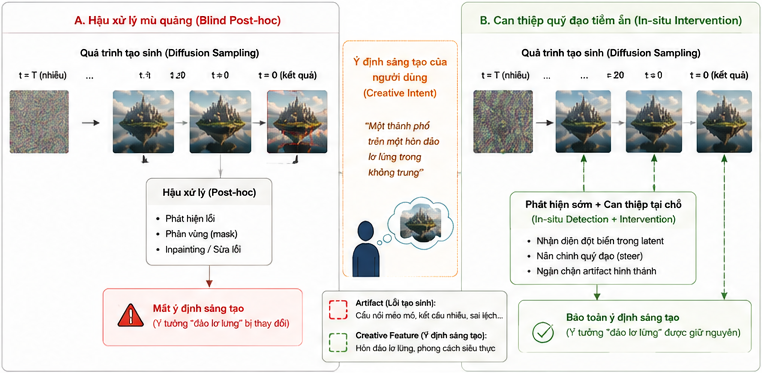
\includegraphics[width=0.9\textwidth]{figures/fig_problem.png} %[span_35](start_span)[span_35](end_span)
    \caption{Minh họa bài toán Intent-aware In-Situ Anomaly Correction: Biểu diễn sự khác biệt giữa việc hậu xử lý mù quáng (blind post-hoc) và can thiệp quỹ đạo tiềm ẩn trực tiếp để bảo vệ ý định sáng tạo nguyên bản của người dùng (Creative Intent).}
    \label{fig:intro_problem} %[span_36](start_span)[span_36](end_span)
\end{figure}

\section{Lý do thực hiện đề tài}
\label{sec:rationale} %[span_37](start_span)[span_37](end_span)

\noindent \textbf{Thứ nhất, ý nghĩa khoa học:} Đề tài đóng góp một khung bài toán hoàn toàn mới, chuyển dịch từ việc "xóa lỗi hậu kỳ" sang việc can thiệp động học "tại chỗ" (in-situ), giúp phân tách rõ ràng giữa ý định văn bản (Textual Intent) và quy luật vật lý. %[span_38](start_span)[span_38](end_span)

\noindent \textbf{Thứ hai, ý nghĩa kỹ thuật:} Việc can thiệp trực tiếp vào quỹ đạo của hàm score trong suy luận (Temporal-Spatial Dynamic Score Correction) mang lại khả năng ngăn chặn lỗi theo thời gian thực mà không cần chạy lại các vòng lặp VCoT đắt đỏ. %[span_39](start_span)[span_39](end_span)

\noindent \textbf{Thứ ba, ý nghĩa thực tiễn:} Các kết quả của luận án sẽ thúc đẩy các hệ thống tạo sinh đạt độ tin cậy cao hơn cho công nghiệp sáng tạo nội dung số chuyên nghiệp, nơi ý định nghệ thuật phải được đặt lên hàng đầu. %[span_40](start_span)[span_40](end_span)

\section{Mục tiêu nghiên cứu}
\label{sec:objectives} %[span_41](start_span)[span_41](end_span)

Mục tiêu tổng quát là xây dựng một pipeline can thiệp bất thường (In-situ Anomaly Steering) cho mô hình tạo sinh, có khả năng phát hiện lỗi từ trong không gian tiềm ẩn và chỉnh sửa thích ứng mà không làm thay đổi ý định của người dùng. %[span_42](start_span)[span_42](end_span)

\noindent \textbf{Các mục tiêu cụ thể:} %[span_43](start_span)[span_43](end_span)
\begin{itemize}
    \item \textbf{MT1 -- Phân tách Ý định (Intent Disentanglement):} Phát triển mô hình biểu diễn kép để phân biệt giữa vi phạm quy tắc vật lý thế giới thực và vi phạm do chủ đích của văn bản (Prompt).
    \item \textbf{MT2 -- Bắt giữ Đột biến (Mutation Trapping):} Khai thác bản đồ chú ý chéo (cross-attention maps) để phát hiện sự phân kỳ của đa tạp nội suy ngay tại các bước thời gian $t$ cụ thể trong quá trình khuếch tán. %[span_44](start_span)[span_44](end_span)
    \item \textbf{MT3 -- Can thiệp Quỹ đạo (Trajectory Steering):} Thiết kế cơ chế trừu tượng hóa và áp dụng vector định hướng (Counterfactual Steering) nhằm nắn chỉnh lại quỹ đạo tạo sinh mà không cần inpainting hậu kỳ. %[span_45](start_span)[span_45](end_span)
\end{itemize}

\section{Tổng quan tình hình nghiên cứu}
\label{sec:literature_review} %[span_46](start_span)[span_46](end_span)

\subsection{Các phương pháp phát hiện bất thường}
Việc phát hiện bất thường hiện nay được chia thành nhóm phân loại có giám sát và không giám sát. Công trình SynArtifact~\cite{cao2024synartifact} đã tinh chỉnh mô hình VLM để phân loại 13 loại bất thường khác nhau. %[span_47](start_span)[span_47](end_span)[span_48](start_span)[span_48](end_span) Tuy nhiên, chúng chỉ giới hạn ở ảnh tĩnh đã hoàn thiện.

\subsection{Suy luận nhận thức và bộ dữ liệu đánh giá}
Các hệ thống suy luận ý nghĩa như AnomReason~\cite{anomreason2024} bắt đầu đề cập đến việc đánh giá bất thường bằng cấu trúc bộ bốn nhân quả. %[span_49](start_span)[span_49](end_span)[span_50](start_span)[span_50](end_span) Song song đó, các nghiên cứu về đánh giá tự động đang liên tục được hiệu chỉnh qua các giao thức nghiên cứu người dùng (Human Studies) để đo lường cảm nhận. %[span_51](start_span)[span_51](end_span)

\subsection{Các phương pháp sửa lỗi (Correction Methods)}
Diffusion Inpainting (ví dụ như Tabatabaei et al.~\cite{tabatabaei2024conditional}) và các mô hình xử lý như ASCED~\cite{asced2024} là các hướng tiếp cận tiêu biểu. %[span_52](start_span)[span_52](end_span)[span_53](start_span)[span_53](end_span) Gần đây nhất, GenShield~\cite{genshield2024} đã thiết lập một tiêu chuẩn mới với pipeline hậu xử lý (post-hoc) dựa trên Mixture-of-Transformers và Visual Chain-of-Thought (VCoT). Dù GenShield rất thành công trong việc sửa các lỗi vật lý, phương pháp này dùng điểm dừng dựa trên "tính bình thường" của ảnh, khiến nó hoàn toàn thất bại trong việc bảo tồn các ý định tạo sinh mang tính dị thường hoặc siêu thực (Surrealism intent). Đề tài này đề xuất một hướng đi hoàn toàn khác: can thiệp trực tiếp vào quá trình sinh (in-situ) thay vì chờ ảnh lỗi để sửa.

\section{Nội dung nghiên cứu}
\label{sec:research_content} %[span_54](start_span)[span_54](end_span)

Đề tài được triển khai qua ba nội dung nghiên cứu gắn liền với ba thành phần cốt lõi của pipeline thống nhất. %[span_55](start_span)[span_55](end_span)

\begin{figure}[htbp] %[span_56](start_span)[span_56](end_span)
    \centering
    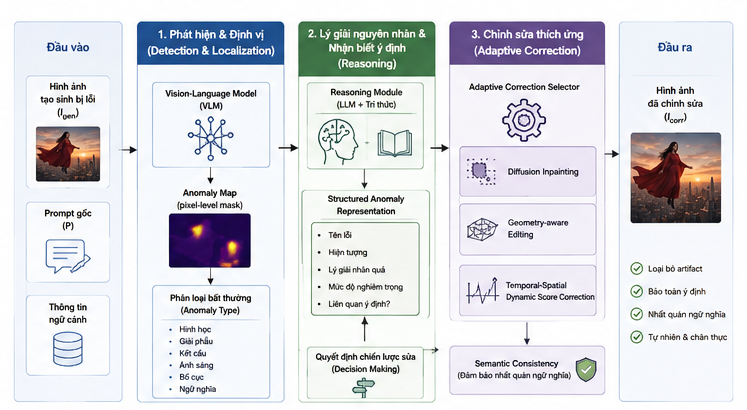
\includegraphics[width=\textwidth]{figures/fig_pipeline.png} %[span_57](start_span)[span_57](end_span)
    \caption{Tổng quan kiến trúc hệ thống (Pipeline) tích hợp 3 module cốt lõi: Phân tách ý định (Intent Disentanglement), Bắt giữ đột biến (Mutation Trapping Detection), và Can thiệp nắn chỉnh quỹ đạo (In-situ Trajectory Steering).}
    \label{fig:overall_pipeline} %[span_58](start_span)[span_58](end_span)
\end{figure}

\subsection{Nội dung 1: Khung phân tách ý định sáng tạo và lỗi tạo sinh (Intent-Conditioned Disentanglement)}
\noindent \textbf{Mục tiêu:} Giải quyết triệt để vấn đề "Feature vs. Bug" bằng cách phân tách nội dung hình ảnh thành hai thành phần: tiền thức vật lý của thế giới và ranh giới ngữ nghĩa của câu lệnh (prompt).

\noindent \textbf{Phương pháp:} Xây dựng một kiến trúc phân nhánh kép (dual-branch representation). Quá trình phát hiện bất thường trở thành một bài toán tối ưu: \textit{Liệu đặc trưng hình học này có vi phạm quy luật vật lý MÀ KHÔNG được cấp phép bởi ngữ nghĩa của Prompt $P$ hay không?} Điều này đảm bảo mô hình không chỉnh sửa các yếu tố phi thực tế nếu người dùng đã cố tình yêu cầu. Xây dựng taxonomy thống nhất cho các lỗi vi phạm loại này. %[span_59](start_span)[span_59](end_span)

\begin{figure}[htbp] %[span_60](start_span)[span_60](end_span)
    \centering
    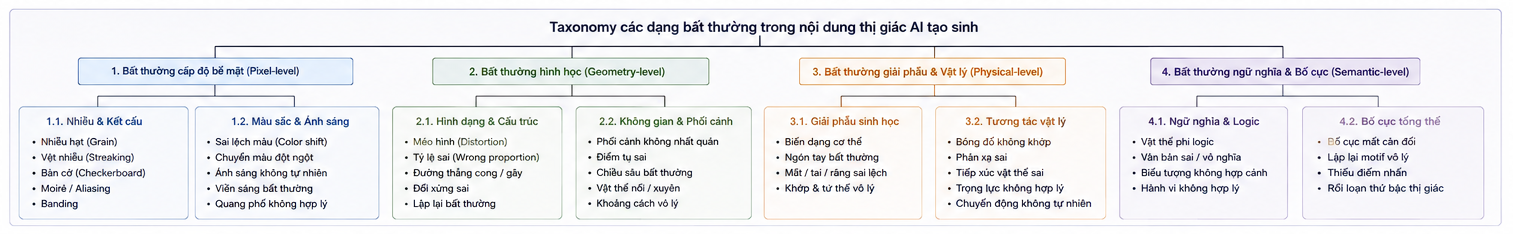
\includegraphics[width=0.95\textwidth]{figures/fig_taxonomy.png} %[span_61](start_span)[span_61](end_span)
    \caption{Cấu trúc phân tầng (Taxonomy) định hướng ý định: Phân loại các vi phạm vật lý không mong muốn so với các biến đổi hình học do chủ đích sáng tạo của prompt.}
    \label{fig:taxonomy} %[span_62](start_span)[span_62](end_span)
\end{figure}

\subsection{Nội dung 2: Bắt giữ đột biến trong quỹ đạo không-thời gian (Mutation Trapping in Temporal-Spatial Dynamics)}
\noindent \textbf{Mục tiêu:} Thay vì chờ đợi ảnh tạo ra bị lỗi, module này nhằm chẩn đoán và phát hiện sớm các dị thường xuất hiện trong không gian tiềm ẩn (latent space) ở các bước thời gian khuếch tán.

\noindent \textbf{Phương pháp:} Phân tích bản đồ Cross-Attention và Latent Gradients tại bước thời gian $t$. Hệ thống sẽ xác định thời điểm hàm score bị kẹt (Mutation Phase) khi cố gắng biểu diễn một khái niệm phức tạp~\cite{cao2025temporal}, từ đó hình thành tín hiệu kích hoạt cho việc nắn chỉnh quỹ đạo trước khi "đột biến" kịp đông đặc thành artifact trên bề mặt pixel. %[span_63](start_span)[span_63](end_span)[span_64](start_span)[span_64](end_span)

\subsection{Nội dung 3: Can thiệp nắn chỉnh quỹ đạo bằng Prompt phản thực tế (Counterfactual Trajectory Steering)}
\noindent \textbf{Mục tiêu:} Sửa chữa ảnh mà không cần dùng đến các kỹ thuật Inpainting cắt dán hậu kỳ (post-hoc masking), đảm bảo tính nhất quán (Semantic Consistency) và bảo vệ phong cách toàn cục của ảnh. %[span_65](start_span)[span_65](end_span)

\noindent \textbf{Phương pháp:} Phát triển một khuôn khổ lập luận phản thực tế (Counterfactual Reasoning). Khi phát hiện đột biến (từ Nội dung 2), mô hình tự động sinh ra một "Prompt phản thực tế" ($P_{cf}$) mô tả chính xác trạng thái lỗi hiện tại. Cơ chế chỉnh sửa lúc này là một phép toán trừ/cộng ngữ nghĩa (semantic arithmetic) trong không gian tiềm ẩn bằng các Vector định hướng (Steering Vectors): loại bỏ embedding của artifact ($P_{cf}$) và cộng dồn sức mạnh của intent nguyên bản ($P$). %[span_66](start_span)[span_66](end_span)

\section{Một số kết quả sơ khởi}
\label{sec:preliminary_results} %[span_67](start_span)[span_67](end_span)

Để chuẩn bị cho luận án, ứng viên đã thực hiện các bước đệm quan trọng: %[span_68](start_span)[span_68](end_span)

\noindent \textbf{1. Nghiên cứu tiền đề về động lực học hàm score:} %[span_69](start_span)[span_69](end_span)
Đã triển khai thực nghiệm phân tích hiện tượng "Mutation Trapping" trong quá trình lấy mẫu của mô hình Diffusion, xác định được các mốc thời gian gây gián đoạn cục bộ dẫn đến artifact cấu trúc. %[span_70](start_span)[span_70](end_span)

\noindent \textbf{2. Xử lý mô hình đa thể thức phân tách ý định:} 
Ứng viên đã tiến hành thử nghiệm các mô hình nền tảng đa thể thức nhằm trích xuất thông tin nhân quả (causal graph) từ prompt và hình ảnh, chứng minh sự tồn tại của mâu thuẫn giữa quy tắc vật lý và ý định người dùng (Feature vs Bug concept). %[span_71](start_span)[span_71](end_span)

\section{Kế hoạch nghiên cứu}
\label{sec:plan} %[span_72](start_span)[span_72](end_span)

Luận án dự kiến thực hiện trong \textbf{04 năm}, phân bổ như sau: %[span_73](start_span)[span_73](end_span)

\paragraph{Năm 1: Khảo sát, phân loại và xây dựng khung phân tách ý định (Nội dung 1):}
Xây dựng taxonomy; thu thập, chuẩn hóa bộ dữ liệu. Phát triển mô hình Intent Disentanglement đầu tiên. Công bố 01 bài báo hội nghị/quốc tế. %[span_74](start_span)[span_74](end_span)

\paragraph{Năm 2: Nghiên cứu động học không-thời gian (Nội dung 2):}
Phân tích hiện tượng Mutation Trapping trong Diffusion, trích xuất đặc trưng chú ý chéo (cross-attention) để cảnh báo sớm. Công bố 1-2 bài báo quốc tế (nhóm CVPR/ECCV/Q1). %[span_75](start_span)[span_75](end_span)

\paragraph{Năm 3: Phát triển mô hình can thiệp In-situ và tích hợp (Nội dung 3):}
Hoàn thiện thuật toán Counterfactual Trajectory Steering. Tối ưu hóa pipeline tổng thể. Công bố 1-2 bài báo quốc tế chất lượng cao. %[span_76](start_span)[span_76](end_span)

\paragraph{Năm 4: Đánh giá diện rộng và bảo vệ luận án:}
Mở rộng thực nghiệm, thực hiện các giao thức đánh giá với người dùng (Human Studies). Hoàn thiện bản thảo luận án, công bố mã nguồn và bảo vệ thành công luận án Tiến sĩ. %[span_77](start_span)[span_77](end_span)

\begin{figure}[htbp] %[span_78](start_span)[span_78](end_span)
    \centering
    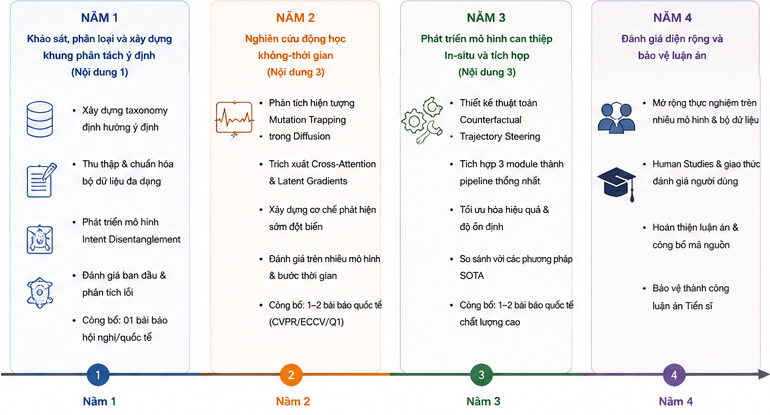
\includegraphics[width=1.0\textwidth]{figures/fig_plan.png} %[span_79](start_span)[span_79](end_span)
    \caption{Lộ trình và kế hoạch nghiên cứu chi tiết 04 năm của đề tài luận án Tiến sĩ, ánh xạ với các mô-đun can thiệp In-situ mới và sản phẩm khoa học đầu ra dự kiến.}
    \label{fig:research_plan} %[span_80](start_span)[span_80](end_span)
\end{figure}

\section{Tài liệu tham khảo} %[span_81](start_span)[span_81](end_span)

\begingroup %[span_82](start_span)[span_82](end_span)
\setlength{\emergencystretch}{8em} %[span_83](start_span)[span_83](end_span)
\setstretch{1.03} %[span_84](start_span)[span_84](end_span)
\leavevmode\printbibliography[heading=none] %[span_85](start_span)[span_85](end_span)
\justifying %[span_86](start_span)[span_86](end_span)
\endgroup %[span_87](start_span)[span_87](end_span)

\end{document}